\section{108 --- Convert Sorted Array to Binary Search Tree}
Given an array $A$ where elements are sorted in ascending order, convert it to a height balanced BST.

For this problem, a height-balanced binary tree is defined as a binary tree in which the depth of the two subtrees of every node never differ by more than 1.
\paragraph{Example:}
\begin{flushleft}
\textbf{Input} : \fcj{A = (-10,-3,0,5,9)},


One possible answer is: \fcj{[0,-3,9,-10,null,5]}, which represents the following height balanced BST:

\begin{figure}[H]
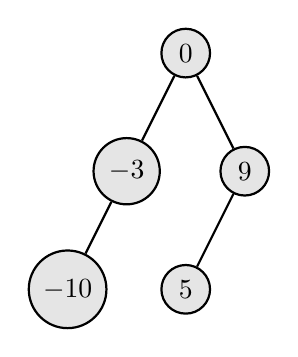
\begin{tikzpicture}
[every node/.style={draw, circle, fill=gray!20!, minimum size=5mm},
%level 1/.style={sibling distance=25mm},
%level 2/.style={sibling distance=15mm},
thick]
\node{0}
child{node{$-3$} child{node{$-10$}} child[missing]}
child{node{9} child{node{5}} child[missing]};
\end{tikzpicture}
\end{figure}



 \end{flushleft}
 \subsection{Recursion}
 同样需要一个递归函数制定构建二叉树的范围,首先找到当前范围的中间位置,以中间位置的值作为当前tree的根,然后中间位置往左的部分即为左子树,中间位置往右的部分为右子树。
%\setcounter{algorithm}{0}
%\begin{algorithm}[H]
%\caption{Recursion}
%\begin{algorithmic}[1]
%\Procedure{SortedArrayToBST}{$A, L$}
%\State \Return $\texttt{CreateTree}(A, 0, L-1)$ \Comment Create BST for $A[0,\ldots, L-1]$
%\EndProcedure
%\end{algorithmic}
%\end{algorithm}
%\texttt{CreateTree}根据给定的有序数组$A$及其范围$[\alpha, \beta]$构建出一个二叉搜索树
%\begin{algorithm}[H]
%\caption{Recursively Build Binary Search Tree}
%\begin{algorithmic}[1]
%\Function{CreateTree}{$A, \alpha, \beta$}
%\If{$\alpha > \beta$}
%\State \Return \texttt{null}
%\EndIf
%\State $M:=(\alpha+\beta)/2$ \Comment The midpoint
%\State Create tree node $T$ with value equal to $A[M]$
%\State $\texttt{LEFT}(T)\gets \texttt{CreateTree}(A, \alpha, M-1)$ \Comment Build left child tree for $A[\alpha, M-1]$
%\State $\texttt{RIGHT}(T)\gets \texttt{CreateTree}(A, M+1, \beta)$ \Comment Build right child tree for $A[M+1, \beta]$
%\State \Return $T$
%\EndFunction 
%\end{algorithmic}
%\end{algorithm}